The \ac{TTR} is an important measure for the effectivity of many pharmacological therapies. \ac{TTR} describes the time in which a patient during a drug treatment has an effective mirror in target range. In this range the patient will experience the desired clinical effect with a minimum of undesirable adverse drug reactions. 

Coumarine derivates are a group of drugs with a similiar structure like Vitamine K. They interfere with the metabolism of Vitamine K as competetive \ac{VKA}. \ac{VKA} inhibit the Vitamine K dependent $\gamma$-carboxilation of the blood clotting factors II, VII, IX and X in the liver. As a result the clotting factors become inactive and blood clotting is delayed. The reduction of the blood coagulation is measured by the \ac{INR} \cite{Hirsh_1998}. The most important coumarines in human medicine used \ac{VKA} are Phenprocoumon and Warfarine. They are used to prevent intravasal thrombembolism. Patients suffer from chronic atrial fibrilation are at high risk to get thrombembolisms in the atrium of the heart and incur a stroke. The livelong therapy with \ac{VKA} reduce the risk of these complications.

But the required therapeutic dosage of \ac{VKA} has a large interindividual variability. Reasons for this phenomen are that the enzymes, responsible for the metabolism of \ac{VKA}, are highly polymorph \cite{Brehm_2016,  Verhoef_2014}. In addition depends the effectiveness of coumarin derivates on the resorption amd metabolism of the single patient. Many drugs and food interact with the metabolism of \ac{VKA} resulting in an intraindividual day-to-day variability of anticoagulative effect. Figure \ref{inr_panel} shows the variability of   

\begin{figure}
	\centering
	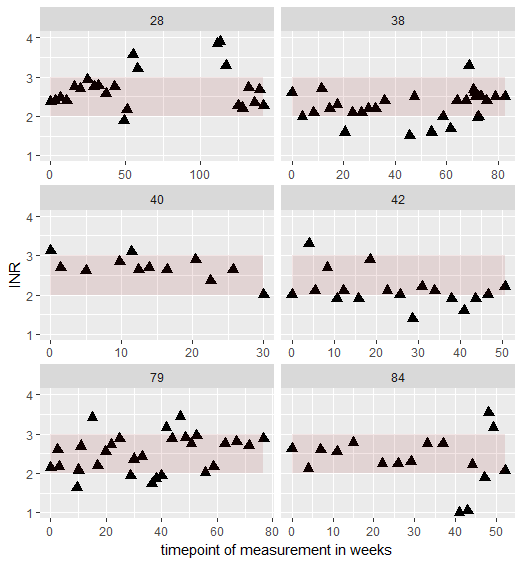
\includegraphics{./images/inr_panel.png}
	\label{inr_panel}
	\caption{Typical INR-Values over time. Lightred area is the therapeutic range}
\end{figure}

    
Two popular methods for therapeutic control of anticoagulation 
Time in therapeutic range assesed by linear interpolation of successive INR measurements
Cross-sectional proportion of all patients' last INR in therapeutic Range
